\let\negmedspace\undefined
\let\negthickspace\undefined
\documentclass[journal]{IEEEtran}
\usepackage[a5paper, margin=10mm, onecolumn]{geometry}
%\usepackage{lmodern} % Ensure lmodern is loaded for pdflatex
\usepackage{tfrupee} % Include tfrupee package

\setlength{\headheight}{1cm} % Set the height of the header box
\setlength{\headsep}{0mm}     % Set the distance between the header box and the top of the text

\usepackage{gvv-book}
\usepackage{gvv}
\usepackage{cite}
\usepackage{amsmath,amssymb,amsfonts,amsthm}
\usepackage{algorithmic}
\usepackage{graphicx}
\usepackage{textcomp}
\usepackage{xcolor}
\usepackage{txfonts}
\usepackage{listings}
\usepackage{enumitem}
\usepackage{mathtools}
\usepackage{gensymb}
\usepackage{comment}
\usepackage[breaklinks=true]{hyperref}
\usepackage{tkz-euclide} 
\usepackage{listings}
% \usepackage{gvv}                                        
\def\inputGnumericTable{}                                 
\usepackage[latin1]{inputenc}                                
\usepackage{color}                                            
\usepackage{array}                                            
\usepackage{longtable}                                       
\usepackage{calc}                                             
\usepackage{multirow}                                         
\usepackage{hhline}                                           
\usepackage{ifthen}                                           
\usepackage{lscape}
\begin{document}
\bibliographystyle{IEEEtran}
\title{4.4.38}
\author{EE25BTECH11002 - Achat Parth Kalpesh }
{\let\newpage\relax\maketitle}
\renewcommand{\thefigure}{\theenumi}
\renewcommand{\thetable}{\theenumi}
\setlength{\intextsep}{10pt} % Space between text and floats
\numberwithin{equation}{enumi}
\numberwithin{figure}{enumi}
\renewcommand{\thetable}{\theenumi}
\parindent 0px


\textbf{Question:}\\
Find the equation of the line which bisects the line segment joining points $\vec{A}\brak{2,3,4}$ and $\vec{B}\brak{4,5,8}$ and is perpendicular to the lines $\frac{x-8}{3} = \frac{y+19}{-16} = \frac{z-10}{7}$ and $\frac{x-15}{3} = \frac{y-29}{8} = \frac{z-5}{-5}$
\textbf{Solution:}\\
Let the equation of the required line be 
\begin{align}
    \vec{x} = \vec{h} + \kappa \vec{m}
\end{align}
where $\vec{h}$ is any point on the line and
$\vec{m}$ is the direction vector of the line\\
Let the direction vectors of the given lines be $\vec{m_1}$ and  $\vec{m_2}$  
\begin{align}
    \vec{m_1} &= \myvec{3\\-16\\7} \\
    \vec{m_2} &= \myvec{3\\8\\-5}
\end{align}
According to the given condition $\vec{h}$ is the midpoint of the line segment joining  $\vec{A}$ and $\vec{B}$ 
\begin{align}
    \vec{h} = \frac{\vec{A} + \vec{B}}{2}
\end{align}
By the given condition,
\begin{align}
    \vec{m_1}^\top\vec{m} &= \vec{0}\\
    \vec{m_2}^\top\vec{m} &= \vec{0}\\
    \myvec{\vec{m_1}^\top \\ \vec{m_2}^\top} \vec{m} &= \vec{0}
\end{align}
\begin{align}
    \myvec{3 & -16 & 7 \\ 3 & 8 & -5}\vec{m} = \vec{0} \xleftrightarrow[]
    {R_2\rightarrow R_2 - R_1} \myvec{3 & -16 & 7 \\ 0 & 24 & -12}\\ 
    \xleftrightarrow[]{R_1\leftarrow R_1 + \frac{2}{3}R_2} \myvec{3 & 0 & -1 \\ 0 & 24 & -12} \xleftrightarrow[]{R_2\leftarrow \frac{R_2}{12}}\myvec{3 & 0 & -1 \\ 0 & 2 & -1}
\end{align}
This yeilds
\begin{align}
    \vec{m} = \myvec{2 \\ 3 \\ 6}
\end{align}
Hence, the vector equation of the line passing through $\vec{h}$ is 
\begin{align}
    \vec{x} &= \vec{h} + \kappa \vec{m}\\
    \vec{x} &= \brak{\frac{\vec{A} + \vec{B}}{2}} + \kappa \vec{m}\\
    \vec{x} &= \brak{\frac{\myvec{2 \\ 3 \\ 4} + \myvec{4 \\ 5 \\ 8}}{2}} + \kappa \vec{m}\\
    \vec{x} &= \myvec{3 \\ 4 \\ 6} + \kappa \myvec{2 \\ 3 \\ 6}
\end{align}

\begin{figure}[h]
    \centering
    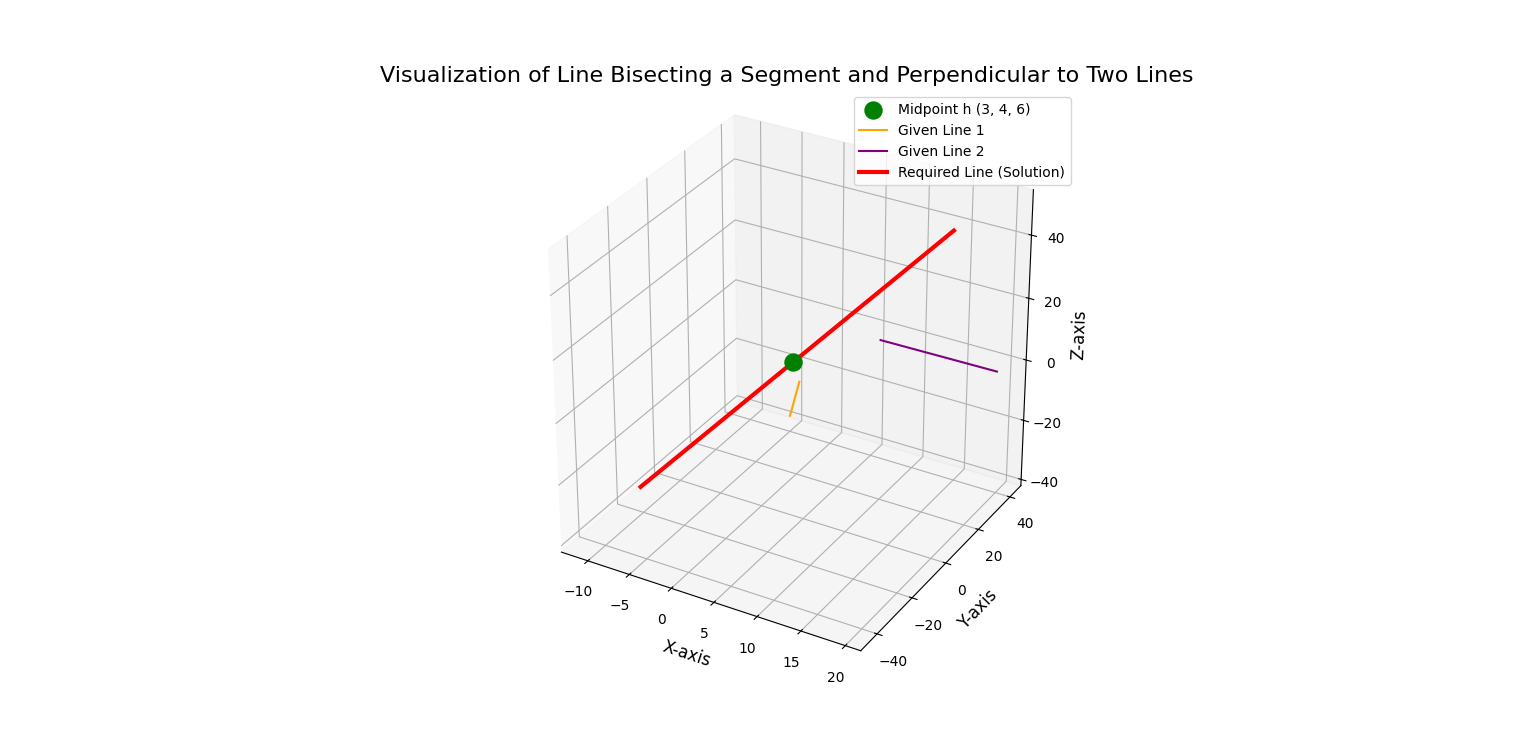
\includegraphics[width=\columnwidth]{figs/figure_py.png}
    \caption{Graph}
    \label{fig:fig}
 \end{figure}
\end{document}